\chapter{Bedienungsanleitung der Anwendung}
\label{Bedienungsanleitung}
Der Programmentwurf besitzt eine mithilfe der Angular-Technologie entwickelte Benutzeroberfläche, deren Anwendung im Folgenden erläutert wird.

\section{Aufrufen der Anwendung}
Die Angular-Anwendung lässt sich mittels des Befehls \code{npm start} im entsprechenden Oberverzeichnis starten.
Nach der Initialisierung ist die Anwendung entsprechend Abbildung \ref{fig:gui-initial-screen} über die Adresse \href{http://localhost:4200}{\code{http://localhost:4200}} erreichbar.

\begin{figure}[H]
	\centering
	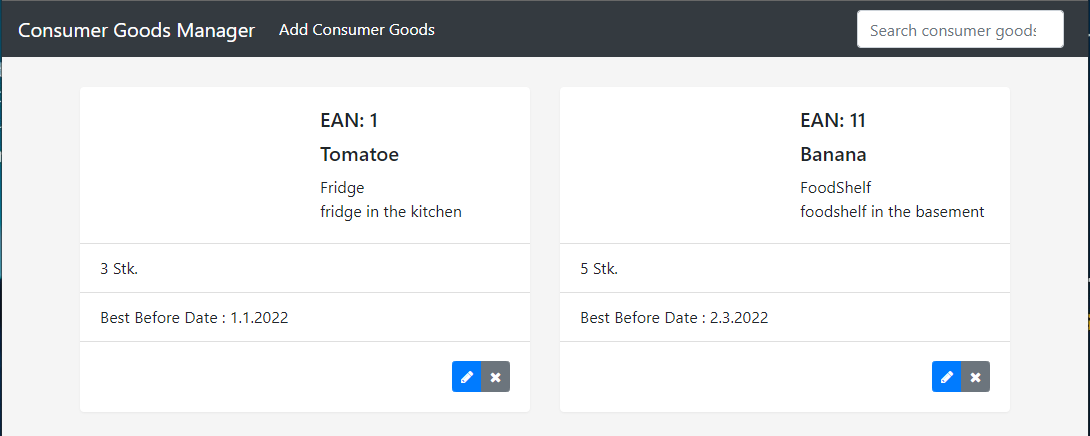
\includegraphics[width=1.0\textwidth]{Bilder/gui/gui-initial-screen.PNG}
	\caption[Grafische Oberfläche des Oberflächenmoduls.]{Die Oberfläche des Oberflächenmoduls zeigt direkt die eingelagerten Konsumgüter samt den jeweiligen Attributen an.}
	\label{fig:gui-initial-screen}
\end{figure}

Auf der initialen Darstellung werden bereits verwaltete Konsumgüter dargestellt.
Wie in Abbildung \ref{fig:gui-search} zu sehen, können über das Eingabefeld an der rechten oberen Seite Konsumgüter entsprechend ihrer Attribute gesucht werden.

\begin{figure}[H]
	\centering
	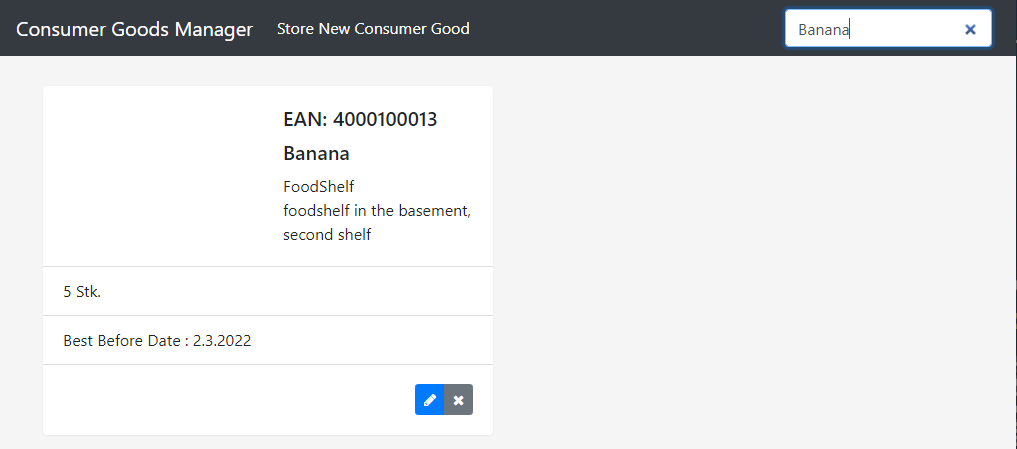
\includegraphics[width=1.0\textwidth]{Bilder/gui/new/gui-search.PNG}
	\caption[Suchfunktion der Oberfläche.]{Über das Eingabefeld auf der rechten oberen Seite kann der Suchbefehl eingegeben werden.}
	\label{fig:gui-search}
\end{figure}

Sollte eine Suchanfrage kein Ergebnis liefern, dann erhält der Nutzer eine Fehlermeldung, wie in Abbildung \ref{fig:gui-search-not-found} dargestellt.
Der gesuchte Befehl kann über das X in der Eingabeleiste gelöscht werden.

\begin{figure}[H]
	\centering
	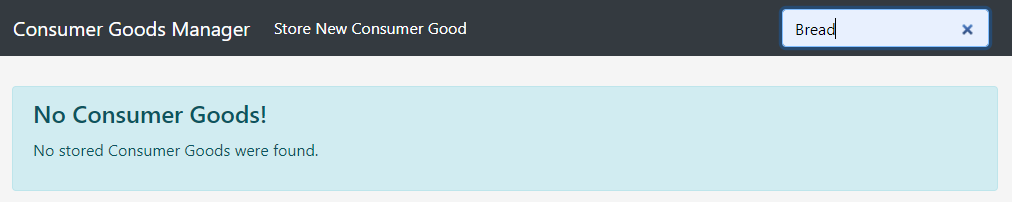
\includegraphics[width=1.0\textwidth]{Bilder/gui/new/gui-search-not-found.PNG}
	\caption[Rückmeldung bei keinem Ergebnis auf Suchanfrage.]{Diese Meldung wird ausgegeben, wenn für den Suchbefehl kein Ergebnis vorliegt.}
	\label{fig:gui-search-not-found}
\end{figure}

\section{Konsumgut anlegen}
\label{konsumgut-anlegen}
Das Anlegen eines Konsumguts ist über den Button \textit{Add Consumer Goods} möglich.
Darauf öffnet sich ein Fenster wie in Abbildung \ref{fig:gui-add-consumer} zur Eingabe der Daten des neuanzulegenden Konsumguts.
Nach Eingabe kann das Konsumgut über den Button \textit{Add Consumer Goods} angelegt werden.

\begin{figure}[H]
	\centering
	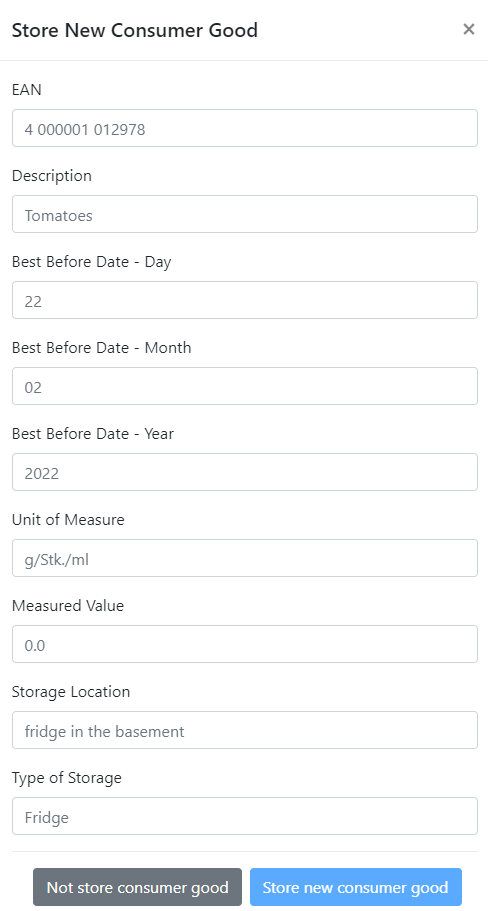
\includegraphics[width=0.3\textwidth]{Bilder/gui/new/gui-store-consumer-goods.PNG}
	\caption[Einlagern eines Konsumguts.]{Eingabemaske zum Eingeben der Attribute eines Konsumguts zum Einlagern.}
	\label{fig:gui-add-consumer}
\end{figure}

Nachdem das Konsumgut angelegt ist, wird es ebenfalls auf der Oberfläche entsprechend Abbildung \ref{fig:gui-created-item} dargestellt.

\begin{figure}[H]
	\centering
	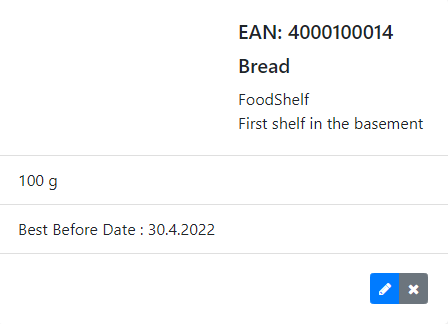
\includegraphics[width=0.3\textwidth]{Bilder/gui/new/gui-created-item.PNG}
	\caption[Darstellung angelegtes Konsumgut.]{Darstellung des Konsumguts nachdem es eingelagert wurde.}
	\label{fig:gui-created-item}
\end{figure}

Über den blauen Button können die Attribute des Konsumguts geändert werden.
Das Vorgehen wird in Abschnitt \ref{konsumgut-aendern} beschrieben.
Über den grauen Button kann das Konsumgut gelöscht werden.
Das Vorgehen wird in Abschnitt \ref{konsumgut-loeschen} beschrieben.

\section{Daten eines Konsumsgut ändern}
\label{konsumgut-aendern}
Zum Ändern von Attributen eines Konsumguts muss der blaue Button des gewünschten Konsumguts ausgewählt werden.
Daraufhin öffnet sich eine Eingabemaske wie in Abbildung \ref{fig:gui-edit} gezeigt, in der die aktuellen Werte der Attribute enthalten sind.
Die Werte können entsprechend angepasst und durch Auswahl des Buttons \textit{Save changes} bestätigt werden.
\begin{figure}[H]
	\centering
	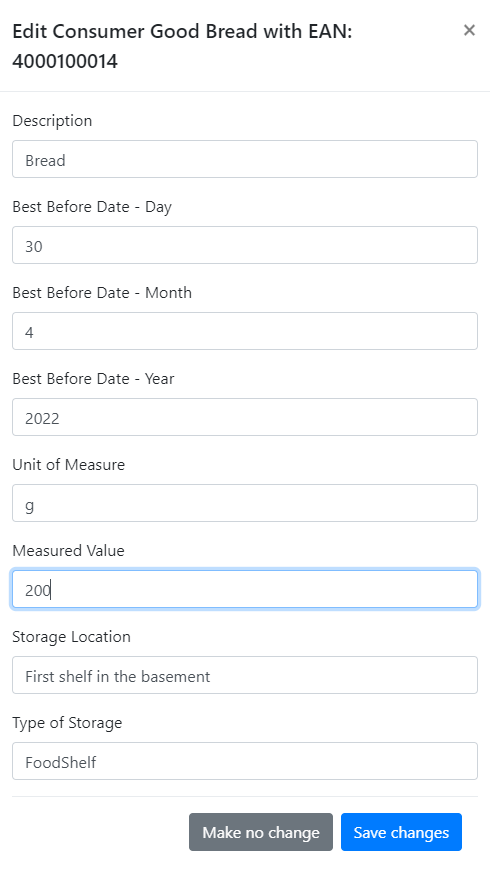
\includegraphics[width=0.3\textwidth]{Bilder/gui/new/gui-edit-consumer-goods.PNG}
	\caption[Daten eines Konsumguts ändern.]{Eingabemaske für das Ändern von Attributen eines Konsumguts.}
	\label{fig:gui-edit}
\end{figure}

\section{Konsumgut löschen}
\label{konsumgut-loeschen}
Das Löschen des Konsumguts erfolgt über den grauen Button.
Bei Auswahl öffnet sich ein Dialogfenster entsprechend Abbildung \ref{fig:gui-delete-item}, dass den Nutzer noch einmal auffordert, den Löschvorgang zu bestätigen, um ein unbeabsichtigtes Löschen zu vermeiden.

\begin{figure}[H]
	\centering
	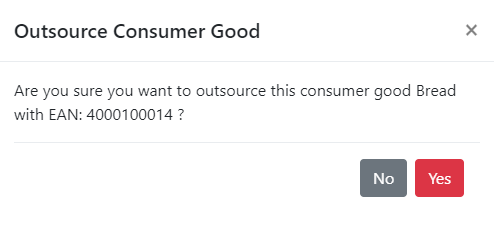
\includegraphics[width=0.7\textwidth]{Bilder/gui/new/gui-outsource-consumer-goods.PNG}
	\caption[Auslagern eines Konsumguts.]{Bestätigungsmeldung für das Auslagern eines Produkts.}
	\label{fig:gui-delete-item}
\end{figure}
